%%%%%%%%%%%%%%%%%%%%%%%%%%%%%%%%%%%%%%%%%%%%%%%%%%%%%%%%%%%%%%%%%%%%%%%%%%%%%%
%% Chinese Journal of Aeronautics three-author TeX template
%% Replace all bracketed example text before submission.
%%%%%%%%%%%%%%%%%%%%%%%%%%%%%%%%%%%%%%%%%%%%%%%%%%%%%%%%%%%%%%%%%%%%%%%%%%%%%%
\documentclass[final,3p,times,twocolumn]{elsarticle}

\usepackage{amsmath,amssymb,amsfonts}
\usepackage{algorithmic}
\usepackage{algorithm}
\usepackage{array}
\usepackage[caption=false,font=footnotesize,labelfont=footnotesize,textfont=footnotesize]{subfig}
\usepackage{textcomp}
\usepackage{stfloats}
\usepackage{bm}
\usepackage{booktabs}
\usepackage{tikz,xcolor}
\usepackage{tabularx}
\usepackage{placeins}
\usepackage{afterpage}
\usepackage{float}
\usepackage[colorlinks=true,linkcolor=blue,citecolor=blue,urlcolor=blue,breaklinks=true]{hyperref}
\captionsetup[subfloat]{font=footnotesize,labelfont=footnotesize,textfont=footnotesize}

\newtheorem{theorem}{Theorem}
\newtheorem{lemma}{Lemma}
\newcommand{\IEEEpubidadjcol}{}
\newcommand{\IEEEPARstart}[2]{{\scshape #1}#2}

%% Superscript numeric citations.
\biboptions{numbers,super,sort&compress}
\setcitestyle{numbers,super,open={},close={},citesep={,}}

%% -------------------------------------------------------------------------
%% CJA PAGE TEXT -- edit these lines directly in this main TeX file.
%% -------------------------------------------------------------------------
\newcommand{\cjapublicationinfo}{Chinese Journal of Aeronautics, (20XX), XX(XX): XXXXXX}
\newcommand{\cjashortauthor}{A et al.}
\newcommand{\cjacorrespondence}{E-mail address: \href{mailto:author.a@example.com}{author.a@example.com} (A).\par E-mail address: \href{mailto:author.c@example.com}{author.c@example.com} (C).}
\newcommand{\cjapeerreviewtext}{Peer review under responsibility of Editorial Committee of CJA.}
\newcommand{\cjapublicationdoi}{https://doi.org/10.1016/j.cja.20XX.XXXXXX}
\newcommand{\cjacopyrighttext}{1000-9361\textcopyright{}20XX The Author(s). Published by Elsevier Ltd on behalf of Chinese Society of Aeronautics and Astronautics.}
\newcommand{\cjalicenseinfo}{[License and open-access information to be supplied by the publisher.]}

\usepackage{cja-manuscript}
\journal{Chinese Journal of Aeronautics}

\begin{document}

\begin{frontmatter}

\title{Full Article Title Written in Sentence Case}

\author[a]{Author A\corref{cor1}}
\ead{author.a@example.com}
\author[b]{Author B}
\ead{author.b@example.com}
\author[a]{Author C\corref{cor2}}
\ead{author.c@example.com}

\affiliation[a]{organization={Department or School, University A},
            city={City A},
            postcode={000000},
            country={Country}}

\affiliation[b]{organization={Department or School, University B},
            city={City B},
            postcode={000000},
            country={Country}}

\cortext[cor1]{Corresponding author.}
\cortext[cor2]{Corresponding author.}

\begin{abstract}
The abstract should identify the research context and the specific problem before presenting the proposed method. It should then summarize the central theoretical or experimental finding, explain its practical significance, and close with the main contribution. Keep the abstract self-contained and use one continuous paragraph. Define every abbreviation at its first occurrence, and ensure that each claim is supported later in the manuscript. Avoid citations, displayed equations, undefined variables, unexplained implementation details, and results that do not appear in the main text.
\end{abstract}

\begin{keyword}
first term \sep
second term \sep
third term \sep
fourth term \sep
fifth term
\end{keyword}

\end{frontmatter}

\section{Introduction}

Introduce the research context and the specific problem addressed by the paper. Explain why the problem matters, summarize the limitations of existing approaches, and identify the gap addressed by this work. Cite the relevant literature in numerical order~\cite{example2026}.

End the introduction with a concise statement of the paper's contributions. Each contribution should correspond to a result established later in the manuscript. A typical organization paragraph may then describe the remaining sections.

\section{Problem Formulation}

Define each symbol before or when it first appears. For example, let $\mathbf{x}\in\mathbb{C}^{N}$ denote the observed signal vector, where $N$ is the number of samples. A generic linear model is
\begin{equation}
  \mathbf{x}=\mathbf{H}\mathbf{s}+\mathbf{n},
  \label{eq:model}
\end{equation}
where $\mathbf{H}$ is the system matrix, $\mathbf{s}$ is the transmitted or latent signal, and $\mathbf{n}$ denotes additive noise.

State the assumptions required by the analysis and distinguish the design model from the experimental setting. Explain the physical meaning of the objective and constraints before presenting the optimization problem.

\begin{figure*}[tbp]
  \centering
  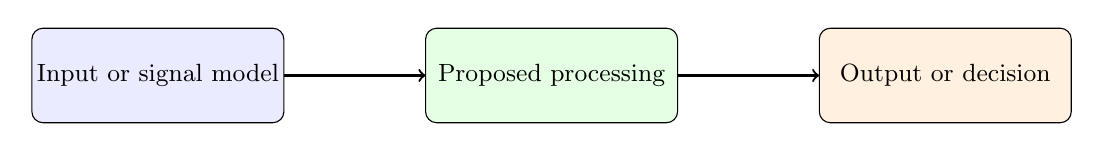
\begin{tikzpicture}[x=1cm,y=1cm,font=\small]
    \draw[rounded corners,fill=blue!8] (0,0) rectangle (3.2,1.2);
    \node at (1.6,.6) {Input or signal model};
    \draw[->,thick] (3.2,.6) -- (5.0,.6);
    \draw[rounded corners,fill=green!10] (5.0,0) rectangle (8.2,1.2);
    \node at (6.6,.6) {Proposed processing};
    \draw[->,thick] (8.2,.6) -- (10.0,.6);
    \draw[rounded corners,fill=orange!12] (10.0,0) rectangle (13.2,1.2);
    \node at (11.6,.6) {Output or decision};
  \end{tikzpicture}
  \caption{Example of a double-column system diagram. Replace this drawing with the paper's first wide figure when needed.}
  \label{fig:system}
\end{figure*}

\section{Proposed Method}

Develop the method in the same order in which its variables are introduced. Give the main derivation, algorithm, or theorem, followed by an interpretation of the result. Clearly state any conditions required for optimality, convergence, or identifiability.

For example, a regularized estimate can be written as
\begin{equation}
  \widehat{\mathbf{s}}
  =\arg\min_{\mathbf{s}}
  \left\|\mathbf{x}-\mathbf{H}\mathbf{s}\right\|_2^2
  +\lambda\left\|\mathbf{s}\right\|_2^2,
  \label{eq:estimate}
\end{equation}
where $\lambda\geq 0$ is the regularization parameter. Explain how the parameter affects the intended engineering tradeoff.

\begin{figure}[tbp]
  \centering
  \subfloat[First condition\label{fig:example_a}]{%
    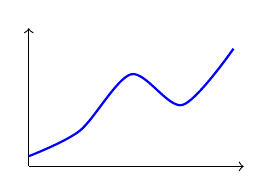
\begin{tikzpicture}[x=.65cm,y=.65cm]
      \draw[->] (0,0) -- (4.2,0);
      \draw[->] (0,0) -- (0,2.7);
      \draw[blue,thick] plot[smooth] coordinates {(0,.2) (1,.7) (2,1.8) (3,1.2) (4,2.3)};
    \end{tikzpicture}}
  \hfill
  \subfloat[Second condition\label{fig:example_b}]{%
    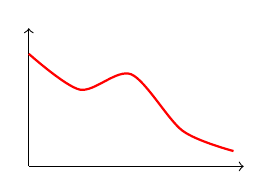
\begin{tikzpicture}[x=.65cm,y=.65cm]
      \draw[->] (0,0) -- (4.2,0);
      \draw[->] (0,0) -- (0,2.7);
      \draw[red,thick] plot[smooth] coordinates {(0,2.2) (1,1.5) (2,1.8) (3,.7) (4,.3)};
    \end{tikzpicture}}
  \caption{Example of two single-column subfigures. Put each subfigure description below its panel.}
  \label{fig:example}
\end{figure}

\section{Results and Discussion}

Describe the data, parameter settings, comparison methods, hardware, software, and evaluation metrics before reporting results. Keep theoretical claims separate from empirical observations, and ensure that every conclusion is supported by a table, figure, or derivation.

\begin{table}[H]
  \centering
  \caption{Example quantitative comparison.}
  \label{tab:example}
  \begin{tabular}{lcc}
    \toprule
    Method & Metric 1 & Metric 2 \\
    \midrule
    Baseline & -- & -- \\
    Proposed method & -- & -- \\
    \bottomrule
  \end{tabular}
\end{table}

Discuss the practical meaning of the results, not only their numerical ordering. State the range of conditions for which the observations apply and avoid extending the conclusion beyond the evaluated evidence.

\section{Conclusions}

Summarize the problem, the central theoretical or methodological result, the practical significance, and the principal limitations in one coherent paragraph. Do not introduce new evidence or repeat a list of numerical values.

\section*{Acknowledgements}
[Insert funding and acknowledgement information.]

\section*{CRediT authorship contribution statement}
\textbf{Author A:} Conceptualization, Methodology, Writing -- original draft. \textbf{Author B:} Investigation, Validation, Data curation, Writing -- review \& editing. \textbf{Author C:} Supervision, Resources, Project administration, Funding acquisition, Writing -- review \& editing.

\section*{Declaration of competing interest}
The authors declare that they have no known competing financial interests or personal relationships that could have appeared to influence the work reported in this paper.

\section*{Data availability}
[Insert the applicable data availability statement.]

\bibliographystyle{cja-num}
\bibliography{template-references}

\end{document}
